\documentclass[aspectratio=169]{beamer}
\usepackage{color,amsmath}
\usepackage{subfigure}
\usepackage{booktabs}
\usepackage{framed}
\usepackage{comment}
\usepackage{hyperref}
\hypersetup{
    colorlinks=true,
    linkcolor=blue
}
\def\vf{\vfill}

%%%%%%%%%%%%%%%%%%%%%%%%%%
\title[]{Mass collaboration}
\author[]{Matthew J. Salganik\\Department of Sociology\\Princeton University}
\date[]{Summer Institute in Computational Social Science\\June 22, 2018
\vfill
\begin{flushleft}
{\scriptsize
The Summer Institute in Computational Social Science is supported by grants from the Russell Sage Foundation and the Alfred P. Sloan Foundation.}
\end{flushleft}
\begin{flushright}

\includegraphics[width=0.1\textwidth]{figures/cc-by.png}
\end{flushright}
}
\begin{document}
%%%%%%%%%%%%%%%%%%%%%%%%%%
\frame{\titlepage}
%%%%%%%%%%%%%%%%%%%%%%%%%%
\begin{frame}

\begin{itemize}
\item 9:15 - 9:30 Welcome and logistics
\item 9:15 - 10:15 Lecture and discussion about mass collaboration
\item 10:15 - 10:30 Break 
\item 10:30 - 12:30 Fragile Families Challenge 
\item 12:30 - 1:30 Lunch
\item 1:30 - 3:30 Fragile Families Challenge
\item 3:30 - 3:45 Group debrief from Fragile Families Challenge 
\item 3:45 - 4:00 Break
\item 4:00 - 5:30 Guest speaker: Sendhil Mullainathan
\item Dinner
\end{itemize}

\end{frame}
%%%%%%%%%%%%%%%%%%%%%%%%%%%
\begin{frame}

Based on feedback, I'm going to cut down on lecture and leave more time for the activity.  For background on mass collaboration, check out Chapter 5 of \textit{Bit by Bit}: \url{https://www.bitbybitbook.com/en/1st-ed/creating-mass-collaboration/}

\end{frame}
%%%%%%%%%%%%%%%%%%%%%%%%%
\begin{frame}

\begin{itemize}
\item Observing behavior
\item Asking questions
\item Running experiments
\item \textcolor{blue}{Creating mass collaboration}
\end{itemize}

\end{frame}
%%%%%%%%%%%%%%%%%%%%%%%%%%%
\begin{frame}

\begin{center}

\includegraphics[width=0.5\textwidth]{figures/wikipedia_logo}
\end{center}

\end{frame}
%%%%%%%%%%%%%%%%%%%%%%%%%%
\begin{frame}

\begin{center}
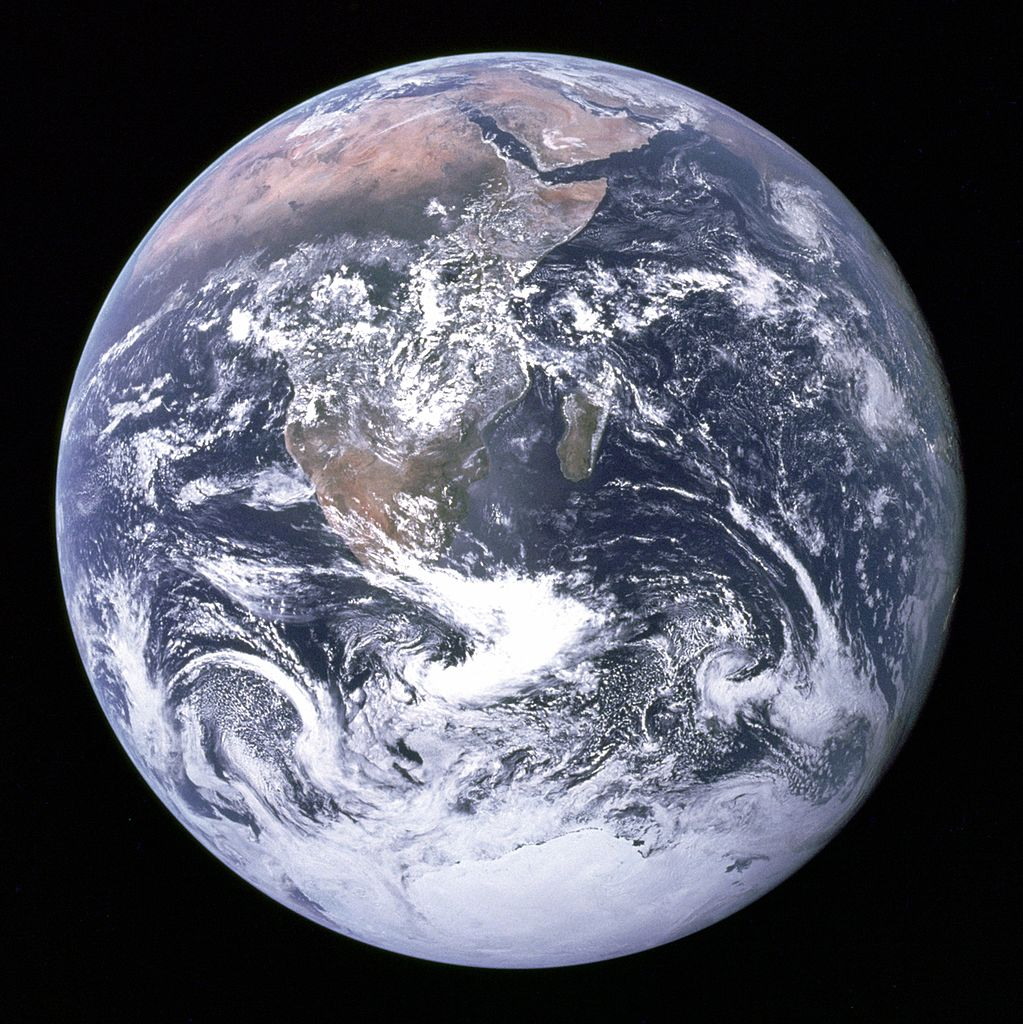
\includegraphics[width=0.5\textwidth]{figures/blue_marble}
\end{center}

\vf
\tiny{\url{https://commons.wikimedia.org/wiki/File:The_Earth_seen_from_Apollo_17.jpg}}

\end{frame}
%%%%%%%%%%%%%%%%%%%%%%%%%%
\begin{frame}

Mass collaboration combines ideas from 
\begin{itemize}
\item crowdsourcing
\item citizen science
\item collective intelligence
\end{itemize}

\end{frame}
%%%%%%%%%%%%%%%%%%%%%%%%%%%
\begin{frame}

\begin{center}
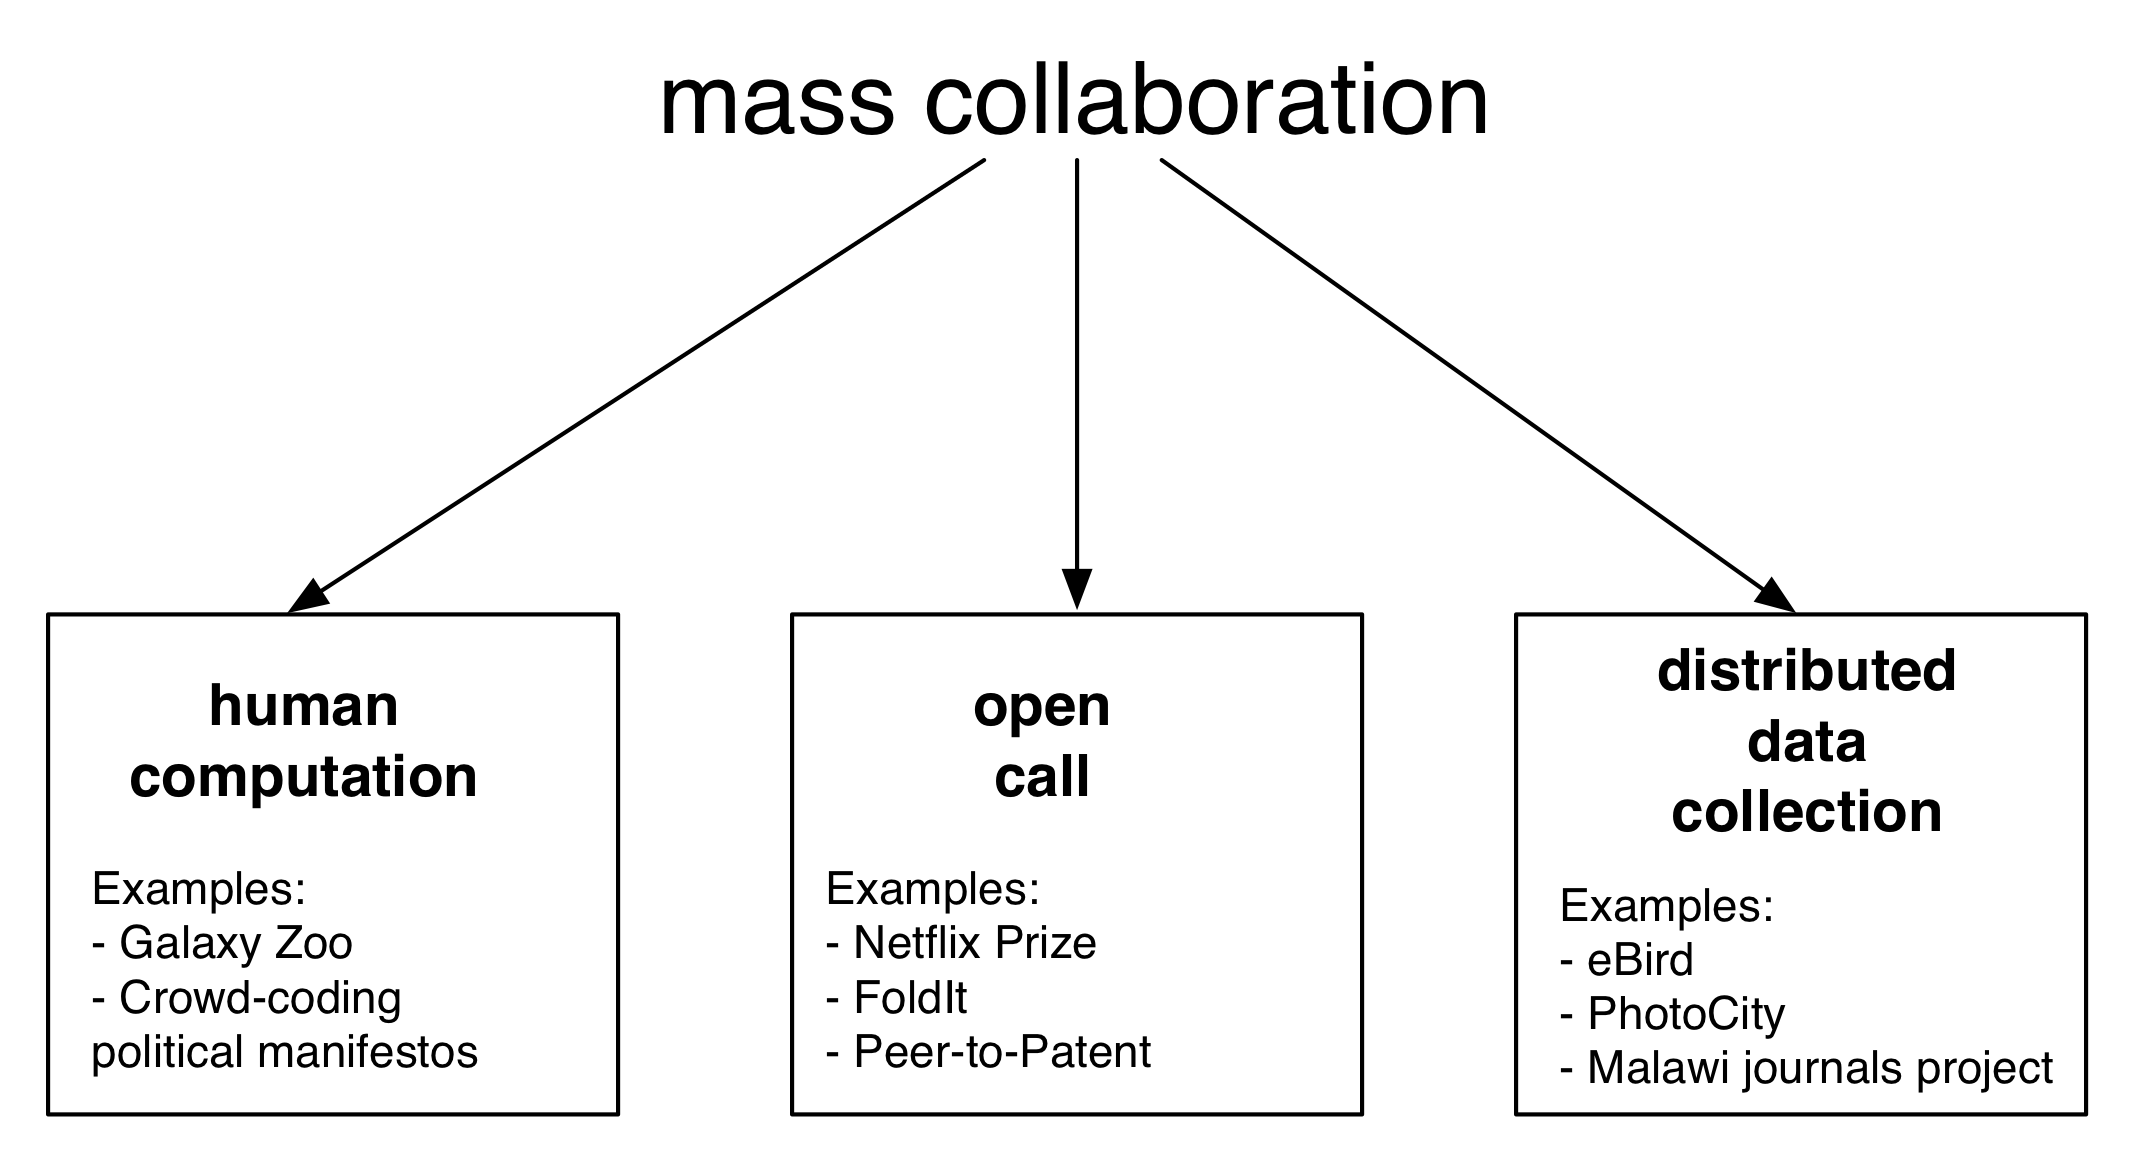
\includegraphics[width=\textwidth]{figures/mass_collaboration_schematic}
\end{center}

\end{frame}
%%%%%%%%%%%%%%%%%%%%%%%%%%
\begin{frame}

Guiding idea:\\
Collaborators not cogs (ornithology and astronomy are examples)

\end{frame}
%%%%%%%%%%%%%%%%%%%%%%%%%%
\begin{frame}

\begin{itemize}
\item Is this really research?
\pause
\item Does this enable new research?
\end{itemize}

\end{frame}
%%%%%%%%%%%%%%%%%%%%%%%%%%
\begin{frame}

\begin{itemize}
\item Is this perfect?
\pause
\item Is this better than we can do without mass collaboration?
\end{itemize}

\end{frame}
%%%%%%%%%%%%%%%%%%%%%%%%%%
\begin{frame}

\begin{itemize}
\item Is this impossible?
\pause
\item Is this possible?
\end{itemize}

\end{frame}
%%%%%%%%%%%%%%%%%%%%%%%%%%
\begin{frame}

An honest assessment: \pause As far as I can tell, most mass collaborations fail

\end{frame}
%%%%%%%%%%%%%%%%%%%%%%%%%%
\begin{frame}

{\Large
\begin{center}
Questions? 
\end{center}
}

\end{frame}
%%%%%%%%%%%%%%%%%%%%%%%%%%

\end{document}
